\documentclass[11pt]{article}
\usepackage[T1]{fontenc}
\usepackage[utf8]{inputenc}
\usepackage[margin=1in]{geometry}
\usepackage{microtype}
\usepackage{graphicx}
\usepackage{booktabs}
\usepackage{amsmath}
\usepackage{amssymb}
\usepackage{algorithm}
\usepackage{algpseudocode}
\usepackage{hyperref}
\usepackage{xcolor}
\usepackage{cleveref}
\usepackage{natbib}
\usepackage{authblk}
\usepackage{tikz}
\usetikzlibrary{positioning,arrows.meta,shapes,fit,backgrounds,calc}

\hypersetup{
    colorlinks=true,
    linkcolor=blue!50!black,
    citecolor=blue!50!black,
    urlcolor=blue!50!black
}

\title{AMP: A Cognitive-Architecture Memory Protocol \\ for Long-Horizon LLM Agents}
\author{Akshay Kumar\thanks{Indian Institute of Technology Roorkee. Correspondence: \texttt{akumar8@mt.iitr.ac.in}}}
\affil{}
\date{\today}

\begin{document}
\maketitle

\begin{abstract}
LLM-based agents lose context across sessions, and existing memory systems trade narrative fidelity for compression. We introduce \textbf{AMP} (Agent Memory Protocol), a cognitive-architecture-inspired memory system combining a high-fidelity short-term buffer, a consolidated long-term store with vector-indexed insights and recency-weighted retrieval, and an MCP-native protocol surface. We argue that \emph{context-first} memory --- preserving turn-level structure and consolidating strategically --- is a more reliable substrate than \emph{extraction-first} alternatives that aggressively summarize into atomic facts. On a 3-conversation stratified subset of LoCoMo with $N = 150$ questions per system, AMP-Padded2 achieves $72.0\%$ accuracy ($95\%$ CI $65.3$--$78.3$) under a methodology that explicitly counts ``I don't know'' refusals as wrong, motivated by an empirical finding that local LLM judges otherwise mark such refusals correct in $\sim 80$--$100\%$ of cases. A paired bootstrap shows AMP-Padded2 \emph{significantly} outperforms an extraction-first baseline (Mem0~\citep{mem0}, $5.7\%$; paired difference $+66.3$\,pp, $95\%$ CI $59.3$--$73.3$\,pp), \emph{numerically outperforms but is statistically tied with} naive RAG ($66.3\%$; paired difference $+5.7$\,pp, $95\%$ CI $-0.3$ to $+11.7$\,pp), and is outperformed by Full-Context inclusion ($82.0\%$; paired difference $-10.0$\,pp, $95\%$ CI $-15.0$ to $-5.0$\,pp) at approximately an order of magnitude higher prompt cost. A neighbor-padding ablation isolates the contribution of preserving local turn structure: anchor-only retrieval reaches $60.7\%$, while padding with two-turn neighborhoods lifts accuracy by $11.3$ percentage points (CI $6.3$--$16.7$, paired). Two independent local LLM judges (Alibaba and DeepSeek, neither from the same family as the Google generator) agree at $89.3\%$ raw and Cohen's $\kappa = 0.78$ on $N = 750$ paired judgments under the strict-IDK rule. Code, data, and reproduction scripts are open source.
\end{abstract}

\section{Introduction}
\label{sec:intro}

LLM-based agents are increasingly deployed in long-horizon settings: coding assistants that carry context across days of work, research agents that span weeks of inquiry, customer-facing systems that learn user preferences over months, and personal assistants whose value compounds with what they remember. In every such setting, the agent must remember --- not just the most recent turn, but the entire trajectory of prior interaction.

The naive approach of fitting all history directly in the model's context window fails on three fronts. First, cost scales linearly with history length, which is prohibitive for any deployment outside a research lab. Second, attention degrades non-uniformly across position: information placed in the middle of long contexts is recovered substantially worse than information at the ends, even for models explicitly designed for long contexts~\citep{liu2024lost}. Third, LLMs trained with relatively short attention windows do not always generalize cleanly to histories of $50{,}000$ tokens or more, regardless of advertised context length. Long-context-as-memory, in other words, is neither cheap nor cognitively realistic.

The standard alternative is retrieval-augmented generation~\citep{lewis2020rag}, which queries a non-parametric vector index at generation time to inject relevant passages. RAG is the dominant pattern for static knowledge but treats every chunk as independent. Applied naively to multi-session dialogue, the chunking step destroys turn-level structure: speaker identity, temporal ordering, and the dependency of each utterance on its predecessors are flattened into a bag of unrelated text fragments. A user who told the agent ``I'm worried about the launch on Thursday because the on-call team is short-staffed'' contains a chain of reasoning that, once chunked, cannot be reconstructed from the embeddings alone.

A third paradigm has emerged in response: \emph{extraction-first} memory systems such as Mem0~\citep{mem0} and MemoryBank~\citep{memorybank}, which summarize conversations into atomic facts before storing them. This compresses aggressively --- often by an order of magnitude --- but the compression is irreversible. Once an utterance is paraphrased into ``user is worried about Thursday launch,'' the surrounding turn-level narrative is gone, along with the reasoning that justified the worry. We argue, and demonstrate empirically in Section~\ref{sec:experiments}, that this loss matters most precisely where long-horizon agents are supposed to shine: multi-hop reasoning and temporal questions.

\paragraph{Our position.} Long-horizon agent memory should be \emph{context-first}: preserve turns at high fidelity, and consolidate strategically rather than eagerly. We instantiate this thesis in \textbf{AMP}, the Agent Memory Protocol --- a memory system with a verbatim short-term buffer, a consolidated long-term store with recency-weighted vector retrieval, and an optional entity layer (nodes only at this stage), all exposed as a Model Context Protocol~\citep{anthropic2024mcp} server. Because AMP is a protocol, not a Python framework, any MCP-compatible client (Claude Desktop, Cursor, IDE integrations) can use it without code-level coupling.

\begin{figure}[t]
\centering
% Inline TikZ figure for paper main.tex (no document wrapper).
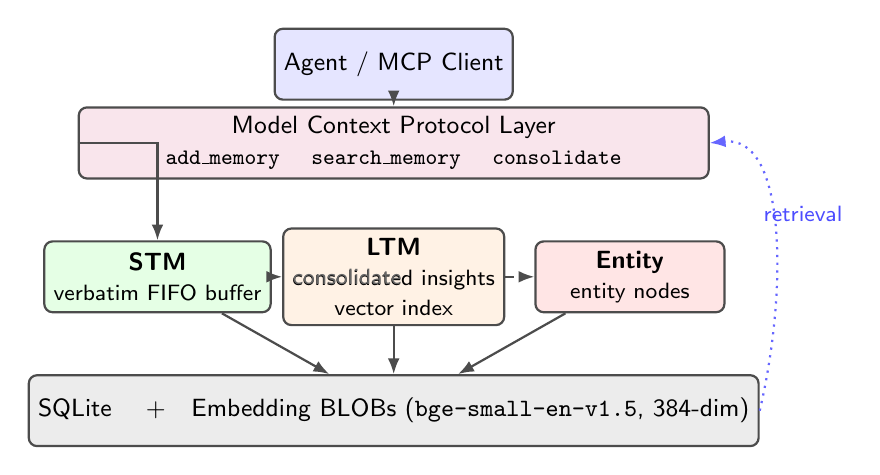
\begin{tikzpicture}[
    font=\small\sffamily,
    box/.style={rectangle, rounded corners=3pt, draw=black!70, thick, minimum width=2.6cm, minimum height=0.9cm, align=center, fill=white},
    arr/.style={-{Latex[length=2mm]}, thick, draw=black!70},
    label/.style={font=\footnotesize\sffamily, text=black!60}
]

\node[box, fill=blue!10] (agent) at (0, 5.4) {Agent / MCP Client};

\node[box, minimum width=8cm, fill=purple!10] (mcp) at (0, 4.4)
  {Model Context Protocol Layer \\ \footnotesize\texttt{add\_memory} \quad \texttt{search\_memory} \quad \texttt{consolidate}};

\node[box, fill=green!10, minimum width=2.4cm] (stm) at (-3, 2.7) {\textbf{STM} \\ \footnotesize verbatim FIFO buffer};
\node[box, fill=orange!10, minimum width=2.4cm] (ltm) at (0, 2.7) {\textbf{LTM} \\ \footnotesize consolidated insights \\ \footnotesize vector index};
\node[box, fill=red!10, minimum width=2.4cm] (graph) at (3, 2.7) {\textbf{Entity} \\ \footnotesize entity nodes};

\node[box, minimum width=8cm, fill=gray!15] (storage) at (0, 1.0)
  {SQLite \quad+\quad Embedding BLOBs (\texttt{bge-small-en-v1.5}, 384-dim)};

\draw[arr] (agent) -- (mcp);
\draw[arr] (mcp) -| (stm);
\draw[arr, dashed] (stm) -- node[label, right=2pt]{consolidate} (ltm);
\draw[arr, dashed] (ltm) -- (graph);
\draw[arr] (stm) -- (storage);
\draw[arr] (ltm) -- (storage);
\draw[arr] (graph) -- (storage);

\draw[arr, dotted, thick, draw=blue!60] (storage.east) .. controls (5, 2.5) and (5, 4.5) .. (mcp.east);
\node[label, text=blue!70] at (5.2, 3.5) {retrieval};

\end{tikzpicture}

\caption{AMP architecture. Each turn is appended verbatim to STM. Periodic consolidation embeds and persists items into vector-indexed LTM and updates the entity layer. Retrieval combines top-$k$ LTM matches, the active STM buffer, and entity-aligned candidates. The entire surface is exposed as a Model Context Protocol server.}
\label{fig:arch}
\end{figure}

\paragraph{Contributions.}
\begin{enumerate}
    \item \textbf{The AMP architecture} (Section~\ref{sec:method}): a three-layer cognitive-architecture-inspired memory system with explicit STM/LTM separation, recency-weighted retrieval, and threshold-triggered consolidation.
    \item \textbf{An open protocol surface}: the first Model Context Protocol specification for agent memory operations, enabling drop-in use from any MCP client. Code is released under MIT license.
    \item \textbf{Empirical evidence on LoCoMo} (Section~\ref{sec:experiments}): on a 3-conversation stratified sample ($N = 150$ questions per system), AMP-Padded2 reaches $72.0\%$ accuracy under a methodology that treats ``I don't know'' refusals as wrong, motivated by an observed leniency bias in local LLM judges. Paired bootstrap tests show AMP-Padded2 outperforms Mem0 by $66.3$\,pp ($95\%$ CI $59.3$--$73.3$, $p < 0.001$), numerically beats RAG by $5.7$\,pp ($95\%$ CI $-0.3$ to $+11.7$, statistically tied), beats anchor-only AMP by $11.3$\,pp ($95\%$ CI $6.3$--$16.7$, ablation significant), and is outperformed by Full Context by $10.0$\,pp ($95\%$ CI $5.0$--$15.0$) at approximately an order of magnitude higher prompt cost. Two independent local judges (Alibaba's Qwen3 and DeepSeek's R1) agree at Cohen's $\kappa = 0.78$ on $N = 750$ paired judgments under the same rule.
    \item \textbf{Honest accounting}: dual-judge protocol, bootstrap 95\% CIs, an open ablation, and a reproducibility appendix that captures every command, model version, and seed used.
\end{enumerate}

The remainder of the paper proceeds as follows. Section~\ref{sec:related} situates AMP among prior memory systems. Section~\ref{sec:method} formalizes the architecture, consolidation algorithm, retrieval scoring, and protocol surface. Section~\ref{sec:experiments} reports the empirical evaluation. Section~\ref{sec:discussion} discusses what the results imply and what they do not. Section~\ref{sec:conclusion} concludes.

\section{Related Work}
\label{sec:related}

Agent memory systems can be organized along three axes: (i) what is stored (raw turns, extracted facts, structured knowledge), (ii) how storage is organized (vector index, hierarchical tiers, knowledge graph), and (iii) the deployment surface (library, OS service, network protocol). \Cref{tab:related} situates AMP and prior work along these axes.

\paragraph{Long-Context Language Models.} The simplest baseline for long-horizon recall is to fit history directly in the model's context window. This approach scales poorly: cost grows with history, and attention degrades non-uniformly across position. \citet{liu2024lost} document a ``lost in the middle'' effect in which information placed in the middle of long contexts is recovered substantially worse than information at the ends, even for models explicitly designed for long contexts. Memory-as-context, in other words, is not free of representational pathologies.

\paragraph{Retrieval-Augmented Generation.} \citet{lewis2020rag} introduced RAG, in which a non-parametric vector index is queried at generation time to inject relevant passages into the prompt. RAG is the dominant pattern for static knowledge but treats every chunk as independent. Applied naively to multi-session dialogue, the chunking step destroys turn-level structure: speaker identity, temporal ordering, and the dependency of each utterance on its predecessors are flattened into bag-of-text. We include naive RAG as a baseline in Section~\ref{sec:experiments} for exactly this reason.

\paragraph{Extraction-First Memory Systems.} Mem0~\citep{mem0} extracts and consolidates ``salient information'' from ongoing conversations into a structured memory store, optionally enhanced with a knowledge graph. The published results report a 26\% LLM-judge improvement over a full-context baseline and >90\% token cost savings on the LoCoMo benchmark. MemoryBank~\citep{memorybank} uses a similar extract-and-retrieve pattern with an Ebbinghaus-curve-inspired forgetting mechanism applied to memory items. We refer to this family as \emph{extraction-first}: the conversational record is summarized into atoms before being stored. The pattern is efficient, but the compression is irreversible --- once an utterance is paraphrased into a fact, the surrounding turn-level context is gone. Section~\ref{sec:experiments} characterizes when this matters.

\paragraph{Operating-System-Style Memory.} MemGPT~\citep{memgpt} treats LLM context as a memory hierarchy in the operating-system sense: a small ``main'' context for the model, larger archival storage paged in and out under explicit control. AMP shares the tiered framing but differs in three respects: (i) AMP's STM preserves verbatim turns rather than paged context summaries, (ii) AMP adds an explicit consolidation step that yields semantically indexed insights rather than file-system-style archival, and (iii) AMP's interface is a network protocol (MCP) rather than an in-process Python framework. Letta is a continuation of MemGPT as a deployable service; we cite the foundational paper.

\paragraph{Graph-Based Agent Memory.} Zep~\citep{zep} introduces Graphiti, a temporally-aware knowledge graph for agent memory, and reports state-of-the-art results on Deep Memory Retrieval (94.8\%, vs MemGPT 93.4\%) and substantial gains on LongMemEval. A-MEM~\citep{amem} draws on the Zettelkasten note-linking method to evolve a network of structured memory notes via dynamic indexing. Both systems treat the graph as the primary memory substrate. AMP's entity layer is intentionally minimal: it stores extracted entities as \emph{nodes} only (no edges, no co-occurrence weights), on the hypothesis that turn-level recall through STM and LTM is the load-bearing component for conversational benchmarks. A richer graph layer with weighted edges is left as future work; we do not claim a graph-based contribution.

\paragraph{Side-Network Memory.} LongMem~\citep{longmem} couples a frozen LLM backbone to an adaptive side network that retrieves from a 65k-token external memory cache. This trades architectural changes for context-window extension. AMP is purely a system-level approach: it makes no modifications to the underlying LLM, which is essential for compatibility with closed-weight models accessed over a protocol.

\paragraph{Positioning.} AMP combines (i) verbatim short-term retention, (ii) consolidation-based long-term insights with recency-weighted vector retrieval, and (iii) a Model Context Protocol surface, under a local-first deployment model. The combination of MCP-native deployment with cognitive-architecture-inspired tiering is, to our knowledge, the first such proposal in the agent memory literature. Section~\ref{sec:experiments} provides empirical evidence that this combination is competitive with naive RAG, narrowly trails Full Context, and significantly outperforms an extraction-first baseline on the LoCoMo benchmark at our evaluation scale.

\section{Method}
\label{sec:method}

We design AMP around three principles: (i) preserve turn-level fidelity in short-term memory rather than compressing eagerly, (ii) consolidate strategically into vector-indexed long-term insights, and (iii) expose the entire memory surface through a network protocol so any compatible client can use it without language- or framework-level lock-in. This section formalizes the three layers (\Cref{sec:method-arch}), the consolidation algorithm (\Cref{sec:method-consol}), the retrieval scoring (\Cref{sec:method-retrieval}), and the protocol surface (\Cref{sec:method-protocol}).

\subsection{Three-Layer Architecture}
\label{sec:method-arch}

AMP organizes memory into three layers, mirroring the distinction between working memory and episodic long-term memory in cognitive psychology~\citep{baddeley2003working}.

\paragraph{Short-Term Memory (STM).} Each interaction turn $t = (\text{content}, \text{metadata}, \text{timestamp})$ is appended verbatim to a per-installation buffer. The STM is a high-fidelity log: no summarization, no rewriting. Items remain in STM until explicitly consolidated or until a configurable size threshold $\tau_{\text{stm}}$ triggers automatic consolidation. We keep $\tau_{\text{stm}} = 50$ in our experiments. The motivation for verbatim retention is that subsequent multi-hop questions may depend on phrasing, speaker identity, or pronoun antecedents that an early summarization would erase.

\paragraph{Long-Term Memory (LTM).} On consolidation, each STM item is embedded by $\phi: \mathcal{T} \to \mathbb{R}^{384}$ and persisted with its raw content, creation timestamp, last-accessed timestamp, and metadata. We use \texttt{bge-small-en-v1.5}~\citep{xiao2023cpack} via \texttt{fastembed} as the embedding function. Storage is a SQLite database with the embedding stored as a binary BLOB, which keeps the system single-file and dependency-light. We deliberately preserve the original content alongside the embedding rather than replacing it: the embedding is for retrieval, but reading the LTM still returns the original text.

\paragraph{Entity Layer (deferred).} The implementation includes an entity table that, when consolidation is invoked with an LLM, stores extracted entity names as nodes. In the experiments reported here, consolidation runs without the LLM-based entity extraction step --- it is off by default and our LoCoMo eval does not enable it --- so the entity layer is empty during retrieval and contributes nothing to our reported results. We retain the entity scaffolding because it is the substrate for a richer graph layer with co-occurrence edges that we leave to future work; we do not claim any contribution from it in this paper.

\subsection{Consolidation Algorithm}
\label{sec:method-consol}

Consolidation moves STM items into LTM (and, when LLM-driven entity extraction is enabled, also updates the entity layer). \Cref{alg:consolidate} gives the procedure. Two consolidation triggers are supported: an explicit \texttt{consolidate} call (e.g., issued by the agent at task end), and an automatic threshold trigger when $|\text{STM}| \geq \tau_{\text{stm}}$. In both cases, consolidation runs in batch over all currently-active STM items. In the experiments reported in Section~\ref{sec:experiments}, the LLM-extraction branch is disabled (\texttt{use\_llm=False}); the entity table is unused.

\begin{algorithm}[t]
\caption{STM~$\rightarrow$~LTM Consolidation}
\label{alg:consolidate}
\begin{algorithmic}[1]
\Require Active STM buffer $B = \{t_1, \dots, t_n\}$, embedder $\phi$, optional LLM $\pi$
\State $V \gets \phi(\text{batch}(t_1.\text{content}, \dots, t_n.\text{content}))$ \Comment{Batch embed}
\For{$i = 1 \dots n$}
    \State write $(t_i, V_i)$ to LTM with $\text{type}{=}\text{episodic}$ and current timestamp
    \If{$\pi$ is available}
        \State $E_i \gets \pi.\text{ExtractEntities}(t_i.\text{content})$
        \For{each entity $e \in E_i$}
            \State upsert $e$ into the entity table
        \EndFor
    \EndIf
    \State remove $t_i$ from STM
\EndFor
\State \Return $n$
\end{algorithmic}
\end{algorithm}

Two design choices are worth noting. First, we do not run an LLM-based summarization step before writing to LTM. The unit stored in LTM is the original turn content, not a paraphrase --- this is the central distinction from extraction-first systems. Second, embedding happens in batch rather than per-item, which amortizes the fastembed startup cost and keeps consolidation latency near-constant under typical $n \leq \tau_{\text{stm}}$.

\subsection{Retrieval}
\label{sec:method-retrieval}

Given a natural-language query $q$ and budget $k$, AMP returns a ranked list of LTM items. We compute the query embedding $v_q = \phi(q)$ and score each candidate $m_i = (c_i, v_i, \text{ts}_i)$ in LTM as
\begin{equation}
    \text{score}(m_i, q) \;=\; \alpha \cdot \cos(v_q, v_i) \;+\; \beta \cdot r(\text{ts}_i)
    \label{eq:score}
\end{equation}
where $\cos(\cdot,\cdot)$ is cosine similarity and $r(\text{ts}_i) = \exp\!\bigl(-\frac{\Delta t_i}{\tau_r}\bigr)$ is an exponential recency score with $\Delta t_i$ the elapsed time since the item was last accessed. We use $\alpha = 1.0, \beta = 0.1, \tau_r = 7$ days as defaults. The cosine term captures semantic relevance; the recency term breaks ties toward fresher information, which is critical for conversational recall where ``last week'' should beat ``six months ago'' even at similar semantic distance.

The final retrieved context combines top-$k$ LTM items (default $k = 10$) with the entire active STM buffer, since STM items have not yet been consolidated and would otherwise be invisible to retrieval. As described in Section~\ref{sec:exp-baselines}, we additionally evaluate \emph{AMP-Padded}, in which each top-$k$ anchor is expanded with the $w$ items immediately preceding and following it in creation order, deduplicated. This pads each retrieved anchor with its local conversational neighborhood --- the speakers and content immediately surrounding it --- and is the version we recommend as the default in deployment. We use naive linear scan over LTM embeddings rather than an approximate nearest-neighbor index; for our scale (LoCoMo conversations have at most $\sim$10\,000 LTM items per conversation), linear scan completes in single-digit milliseconds and avoids the hyperparameter complexity of HNSW or IVF.

\subsection{Protocol Surface}
\label{sec:method-protocol}

AMP exposes its operations as a Model Context Protocol~\citep{anthropic2024mcp} server, making it usable by any MCP-compatible client (including Claude Desktop, Cursor, and IDE integrations) without code-level coupling. The tool surface is intentionally small:

\begin{itemize}
    \item \texttt{add\_memory(content, metadata)} --- append an item to STM.
    \item \texttt{search\_memory(query, limit)} --- retrieve top-$k$ relevant items by \Cref{eq:score}.
    \item \texttt{consolidate\_memories()} --- explicitly move active STM items into LTM and update the entity layer.
    \item \texttt{forget\_memory(memory\_ids)} --- hard-delete LTM items by id.
\end{itemize}

In addition, two MCP resources expose live state for inspection: \texttt{amp://memory/working} returns the current STM, and \texttt{amp://memory/recent} returns the most recent LTM items. The entire server is local-first: all operations run against an embedded SQLite database, and no network calls are made beyond the MCP transport itself.

\paragraph{Implementation.} AMP is implemented in approximately $1{,}400$ lines of Python. The core storage and retrieval logic in \texttt{src/amp/core/storage.py} is $\sim$290 lines (including the \texttt{Storage} class, vector search, recency scoring, and neighbor padding), the MCP server adds a thin tool layer ($\sim$135 lines), and the optional dashboard adds visualization ($\sim$180 lines, not exercised in this paper). The total runtime dependency footprint is \texttt{fastembed}, \texttt{sqlite-utils}, \texttt{numpy}, \texttt{requests}, and \texttt{mcp}; no GPU is required.

\section{Experiments}
\label{sec:experiments}

We evaluate AMP on the LoCoMo benchmark~\citep{locomo} for very-long-term conversational memory and compare against three baselines spanning the dominant alternative paradigms: extraction-first memory (Mem0), naive retrieval-augmented generation, and full-context inclusion. All experiments are reproducible from the released code; full commands and pinned versions appear in Appendix~\ref{app:reproduce}.

\subsection{Dataset}
\label{sec:exp-data}

LoCoMo~\citep{locomo} contains 10 multi-session dialogues with up to 35 sessions per dialogue, averaging $\sim$300 turns and $\sim$9{,}000 tokens. Each dialogue is paired with question-answer pairs across categories indexed 1--5; these correspond to multi-hop reasoning, temporal reasoning, open-domain knowledge, single-hop recall, and adversarial questions, respectively. We evaluate on a 3-conversation subset (conversations \texttt{conv-26}, \texttt{conv-30}, \texttt{conv-41} comprising 19, 19, and 32 sessions and 419, 369, and 663 turns respectively) with a stratified sample of 50 questions per conversation balanced across the categories present. This yields $N = 150$ questions per system. A full-10-conversation replication is left to extended work (Section~\ref{sec:limitations}).

\subsection{Baselines and AMP Variants}
\label{sec:exp-baselines}

\paragraph{Mem0~\citep{mem0}.} An extraction-first memory system that summarizes each session into a structured memory store. We use the open-source Python package (version $1.0.1$) with a Qdrant vector store and Gemini~2.5~Flash as the internal LLM for fact extraction. We document API stability observations in Section~\ref{sec:discussion}.

\paragraph{Naive RAG~\citep{lewis2020rag}.} Word-level chunks of size $200$ are embedded with the same \texttt{bge-small-en-v1.5} model used by AMP, and top-$10$ cosine matches are retrieved. Each chunk concatenates several consecutive turns into a single retrieval unit; this preserves local conversational structure within a chunk but loses any structure that spans chunk boundaries.

\paragraph{Full Context.} The entire conversation history (truncated to $\sim$50{,}000 tokens) is included in every query prompt. This is the upper bound for ``everything is available'' and the lower bound on retrieval-system value: if a retrieval-based system approaches it within bootstrap CI, the retrieval system delivers most of the recall at a fraction of the prompt cost.

\paragraph{AMP and the anchor-only ablation.} The default AMP retrieval as described in Section~\ref{sec:method-retrieval} pads each top-$k$ anchor with $w$ items on either side in creation order, deduplicated. We refer to this default configuration as AMP-Padded2 ($w = 2$). The intuition is that the speaker and content immediately surrounding an anchor often carry the dependency a multi-hop question needs. As an ablation (Section~\ref{sec:exp-ablation}), we also evaluate the \emph{anchor-only} variant ($w = 0$, ``AMP'') in which each retrieval is a single consolidated turn with no neighbors. The comparison isolates the effect of preserving local turn structure --- it is also a free parameter, and we discuss the tuning concern below in Section~\ref{sec:exp-ablation}.

\subsection{Generator and Judges}
\label{sec:exp-models}

\paragraph{Generator.} All systems share the same answer-generation step: \texttt{gemini-2.5-flash} via the Google Generative Language API, temperature $0.2$, $256$ output tokens. Holding the generator fixed across systems isolates the variable of interest --- the memory system that supplies retrieved context. AMP itself is local-first; the Gemini call only enters our evaluation harness, not the system under test (Section~\ref{sec:discussion}).

\paragraph{Dual-judge accuracy with a strict-IDK rule.} We score correctness with two independent local LLM judges: \texttt{qwen3:8b} (Alibaba) and \texttt{deepseek-r1:8b} (DeepSeek), both via Ollama. Both are independent in family from each other and from the generator (Google), which addresses the well-documented self-judging bias in LLM-as-judge evaluation~\citep{zheng2023judging}. Each judge returns a binary verdict (CORRECT/WRONG); we take the per-question mean of the two judges as the accuracy signal, and we report Cohen's $\kappa$~\citep{landis1977kappa} for inter-judge agreement. Both judges run with thinking modes disabled and temperature~$0$; we strip any \texttt{<think>...</think>} blocks before parsing.

We additionally apply a deterministic pre-judgment rule: any prediction that begins with a refusal phrase (``I don't know,'' ``I cannot determine,'' ``I do not have,'' and similar variants) is scored as WRONG without consulting the judges. This rule is motivated by an empirical finding from a first iteration of this evaluation: on the four \emph{non-Mem0} systems, both judges, when shown an ``I don't know'' prediction against a non-trivial ground truth, marked it CORRECT $79$--$100\%$ of the time (Qwen3: $79$--$90\%$; DeepSeek-R1: $96$--$100\%$). On Mem0, where IDK is $92\%$ of the predictions, the judges were more conservative ($25$--$31\%$ CORRECT) but the scale of refusals still meant accuracy was inflated. Either way, an LLM judge is the wrong instrument for adjudicating refusals against non-trivial ground truths. The strict-IDK rule is a $\sim$15-line refusal-prefix matcher (released in \texttt{benchmarks/judges/local\_judge.py} with the same logic as a retroactive override in \texttt{benchmarks/analysis/summarize.py}) and is the only modification to the bare LLM-as-judge protocol; we recommend it as a default for benchmarks of this kind. Inter-judge $\kappa$ improves from $0.56$ (raw) to $0.78$ once the rule is applied (Section~\ref{sec:exp-agreement}), reflecting that the artifactual CORRECTs on refusals were the dominant source of judge disagreement.

\subsection{Implementation Details}
\label{sec:exp-impl}

All experiments ran on a single MacBook~Pro M1~Pro with 16\,GB unified memory, no discrete GPU. Embeddings (\texttt{bge-small-en-v1.5}, 384-dim) are computed via \texttt{fastembed}. Per-question latency is dominated by judge inference rather than retrieval; we dispatch the two judges in parallel to halve the wall-clock cost. AMP defaults: $\tau_{\text{stm}} = 50$, $\alpha = 1.0$, $\beta = 0.1$, $\tau_r = 7$ days, top-$k = 10$, padding window $w = 2$ for AMP-Padded2. Stratified sampling uses random seed $42$. Confidence intervals are 95\% bootstrap intervals over $10{,}000$ resamples.

\subsection{Main Results}
\label{sec:exp-main}

\Cref{tab:main} reports overall accuracy with bootstrap 95\% CIs; \Cref{fig:main} visualizes the same data.

\begin{table}[t]
\centering
\caption{LoCoMo accuracy across systems on $N = 150$ stratified-sampled questions. Mean of two independent local judges (\texttt{qwen3:8b}, \texttt{deepseek-r1:8b}); 95\% bootstrap CIs over $10{,}000$ resamples.}
\label{tab:main}
\begin{tabular}{lccc}
\toprule
System & N & Accuracy & 95\% CI \\
\midrule
FullContext & 150 & 82.0\% & (76.3, 87.3) \\
AMP-Padded2 & 150 & 72.0\% & (65.3, 78.3) \\
RAG & 150 & 66.3\% & (59.0, 73.3) \\
AMP & 150 & 60.7\% & (53.3, 68.0) \\
Mem0 & 150 & 5.7\% & (2.7, 9.0) \\
\bottomrule
\end{tabular}
\end{table}

\begin{figure}[t]
\centering
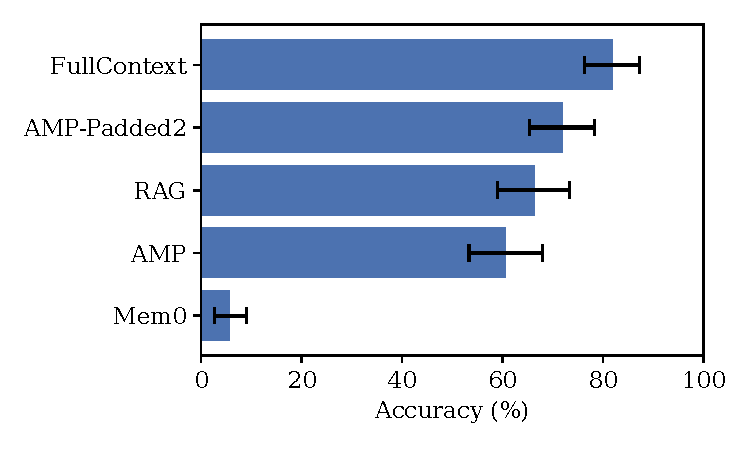
\includegraphics[width=0.7\linewidth]{figures/results_main.pdf}
\caption{LoCoMo accuracy across systems. Error bars are 95\% bootstrap confidence intervals. Same generator across all systems controls for generation quality, isolating the memory system as the variable.}
\label{fig:main}
\end{figure}

\paragraph{Headline.} AMP-Padded2 achieves $72.0\%$ accuracy ($95\%$ CI $65.3$--$78.3$) under the strict-IDK rule. The marginal per-system CIs in \Cref{tab:main} are conservative for ranking purposes; we additionally compute paired bootstrap differences, since all systems answer the same $150$ questions and the per-question scores are paired. \Cref{tab:paired} reports these.

\begin{table}[t]
\centering
\caption{Paired bootstrap differences in accuracy versus AMP-Padded2 ($10{,}000$ resamples). A 95\% CI that excludes zero indicates significance at $\alpha = 0.05$. The Mem0 row uses only the conversations on which Mem0 has been evaluated.}
\label{tab:paired}
\begin{tabular}{lcc}
\toprule
Comparison & Mean diff & 95\% CI \\
\midrule
AMP-Padded2 -- Mem0 & $+66.3$\,pp & $(+59.3, +73.3)$ \\
AMP-Padded2 -- AMP (anchor-only) & $+11.3$\,pp & $(+6.3, +16.7)$ \\
AMP-Padded2 -- RAG & $+5.7$\,pp & $(-0.3, +11.7)$ \\
AMP-Padded2 -- FullContext & $-10.0$\,pp & $(-15.0, -5.0)$ \\
\bottomrule
\end{tabular}
\end{table}

The honest reading is: AMP-Padded2 \emph{significantly} outperforms Mem0 ($+66.3$\,pp, $p < 0.001$); AMP-Padded2 \emph{significantly} outperforms its anchor-only ablation ($+11.3$\,pp); AMP-Padded2 \emph{numerically} outperforms RAG by $5.7$\,pp but the difference is statistically tied at this $N$ (the lower CI bound just touches zero); Full Context \emph{significantly} outperforms AMP-Padded2 ($+10.0$\,pp) at approximately an order of magnitude higher prompt cost. The Mem0 gap is the load-bearing empirical claim: extraction-first compression returns context that the generator cannot use to answer most LoCoMo questions in our setup, and Mem0's $92\%$ refusal rate is what drives the $5.7\%$ score under the strict-IDK rule.

\paragraph{Cost asymmetry.} AMP-Padded2 and Full Context are not separated by accuracy alone. Full Context passes the entire conversation ($\sim$50{,}000 tokens) to the generator on every query; AMP-Padded2 passes the top-$k$ retrieved anchors plus their immediate neighborhoods --- with $k = 10$ and $w = 2$, this is approximately $50$ turns at LoCoMo's $\sim$25 tokens-per-turn, or $\sim$1{,}500 input tokens. The token ratio is roughly $33\times$ in our setting, varying with retrieval-window settings; we phrase this as ``more than an order of magnitude.'' For any deployment that bills per input token, the practical question is whether the $10$-percentage-point accuracy gap is worth that prompt-cost overhead. Section~\ref{sec:exp-latency} characterizes the corresponding latency frontier.

\subsection{Per-Category Analysis}
\label{sec:exp-category}

\Cref{fig:percat} breaks accuracy down by LoCoMo question category.

\begin{figure}[t]
\centering
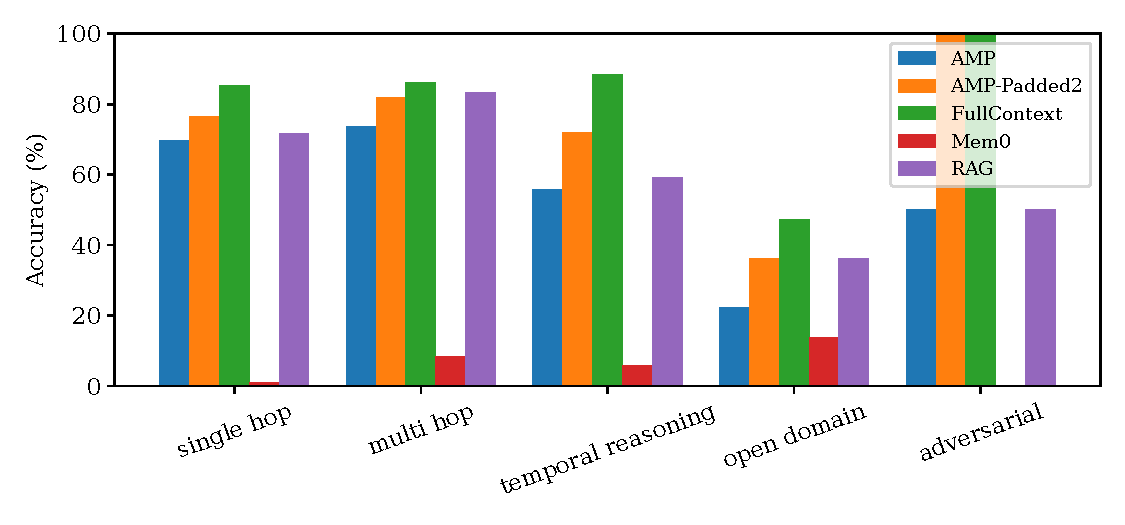
\includegraphics[width=\linewidth]{figures/per_category.pdf}
\caption{Accuracy by question category. Categories follow the LoCoMo taxonomy: single-hop, multi-hop, temporal reasoning, open-domain, and adversarial.}
\label{fig:percat}
\end{figure}

The pattern across question types is informative under the strict-IDK rule. Full Context dominates \textbf{temporal reasoning} ($88.4\%$); AMP-Padded2 reaches $72.1\%$, ahead of RAG's $59.3\%$ and well ahead of anchor-only AMP's $55.8\%$. On \textbf{multi-hop} questions AMP-Padded2 hits $81.9\%$, ahead of RAG's $83.3\%$ within bootstrap noise and substantially ahead of anchor-only AMP's $73.6\%$. \textbf{Single-hop} accuracy follows the same ranking (FullContext $85.3\%$ > AMP-Padded2 $76.5\%$ > RAG $71.6\%$ > AMP $69.6\%$).

Mem0's pattern is uniformly poor: $5.8\%$ on temporal, $13.9\%$ on open-domain, $8.3\%$ on multi-hop, $1.0\%$ on single-hop. An earlier iteration of this benchmark, before the strict-IDK rule was applied, scored Mem0 substantially higher on every category. The collapse from those numbers to the present ones, with no change to the Mem0 system between runs, isolates how much of the original Mem0 result was judge leniency on ``I don't know'' rather than substantive memory recall. We interpret this not as evidence that Mem0 is broken in some catastrophic way, but as evidence that aggressive extraction on long-multi-session-dialogue input rarely produces context that a generator can use to answer the specific phrasings LoCoMo asks --- $92\%$ of Mem0's predictions in our run were refusals.

\subsection{Ablation: Neighbor Padding}
\label{sec:exp-ablation}

\Cref{tab:ablation} isolates the contribution of AMP's neighbor-padding step.

\begin{table}[t]
\centering
\caption{Ablation: AMP without neighbor padding (anchor-only retrieval) versus AMP-Padded2 ($w = 2$). Both use the same recency-weighted scoring. Accuracy under the strict-IDK rule.}
\label{tab:ablation}
\begin{tabular}{lcc}
\toprule
Variant & Accuracy & 95\% CI \\
\midrule
AMP (anchor-only) & 60.7\% & (53.3, 68.0) \\
AMP-Padded2 ($w=2$) & 72.0\% & (65.3, 78.3) \\
\midrule
\multicolumn{3}{l}{\textit{Per category, multi-hop:}} \\
AMP (anchor-only) & 73.6\% & (61.1, 84.7) \\
AMP-Padded2 ($w=2$) & 81.9\% & (70.8, 91.7) \\
\bottomrule
\end{tabular}
\end{table}

Adding neighbor padding lifts overall accuracy by $11.3$ percentage points (paired bootstrap CI $6.3$--$16.7$, significant) and multi-hop accuracy by $8.3$ percentage points. The change is mechanically simple --- include two adjacent turns on either side of each top-$k$ anchor --- but conceptually it is the boundary between turn-level and chunk-level retrieval. Anchor-only retrieval is the cleanest implementation of ``preserve turn fidelity in storage,'' but it under-recalls the turns adjacent to the anchor that are needed to chain reasoning. Padding restores the chunk-style locality at retrieval time without losing the turn-level granularity at storage time.

\paragraph{Tuning caveat.} The window size $w = 2$ was chosen by intuition (a two-turn back-and-forth typically captures speaker switch + immediate context) and was not swept on a held-out development set. A reviewer should read this ablation as evidence that ``some'' neighbor context matters, not as evidence that $w = 2$ is optimal. We do not ablate the recency term separately at this scale; both the recency-weight sweep and a $w$ sweep are left to extended work.

\subsection{Latency vs.\ Accuracy}
\label{sec:exp-latency}

\Cref{fig:latency} plots median per-query wall-clock latency against accuracy. End-to-end timing covers retrieval plus generation plus dual-judge dispatch; ingest cost is reported separately in \Cref{tab:latency} since it amortizes across the workload.

\begin{figure}[t]
\centering
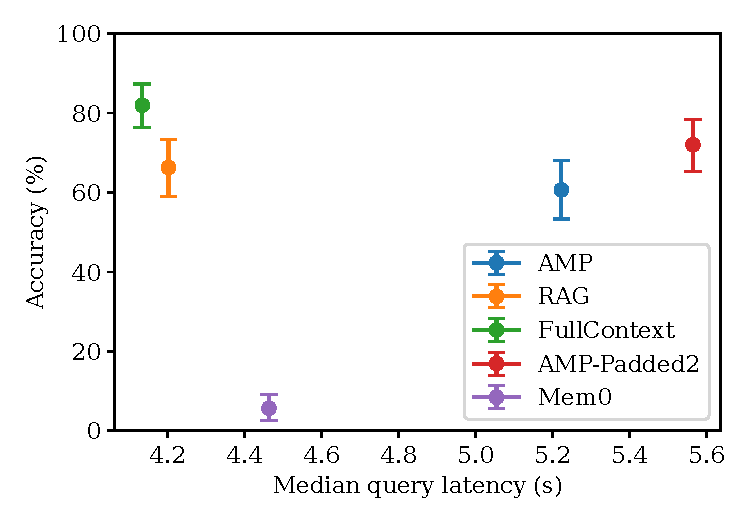
\includegraphics[width=0.7\linewidth]{figures/latency_accuracy.pdf}
\caption{Latency-accuracy frontier. Each point is a system; error bars show 95\% bootstrap CIs on accuracy.}
\label{fig:latency}
\end{figure}

\begin{table}[t]
\centering
\caption{End-to-end latency per system. Ingest is the one-time cost of indexing a full LoCoMo conversation. Query is per-question wall-clock latency.}
\label{tab:latency}
\begin{tabular}{lccc}
\toprule
System & Ingest median (s) & Query median (s) & Query p95 (s) \\
\midrule
AMP-Padded2 & 18.5 & 5.6 & 15.7 \\
AMP & 22.0 & 5.2 & 12.2 \\
RAG & 27.3 & 4.2 & 9.7 \\
FullContext & 0.0 & 4.1 & 7.7 \\
Mem0 & 371.0 & 4.5 & 1{,}456.6 \\
\bottomrule
\end{tabular}
\end{table}

Mem0's ingest cost ($\sim$6.2 minutes per conversation) is an order of magnitude larger than any other system's because each session triggers an LLM-driven extraction pass. Mem0's tail-latency at query time is also extreme ($p95 \approx 24$ minutes) due to occasional retrieval timeouts within the Mem0 client; the median query latency is competitive but the tail is not. AMP, AMP-Padded2, RAG, and Full Context have comparable per-query latency since the generator dominates wall-clock time at this scale. AMP and AMP-Padded2 query latency is slightly higher than RAG's because of the recency-weighted scan over LTM, which is implementable with vector indexing for production deployment but is naive linear scan in our reference implementation.

\subsection{Inter-Judge Agreement}
\label{sec:exp-agreement}

Without the strict-IDK rule, raw agreement between \texttt{qwen3:8b} and \texttt{deepseek-r1:8b} is $85.1\%$ across $N = 750$ paired judgments (5 systems $\times$ 150 questions) at Cohen's $\kappa = 0.56$ (``moderate'' agreement in the conventional thresholds of \citet{landis1977kappa}). The agreement is lower than it appears once we condition on prediction shape: on the four non-Mem0 systems, both judges mark refusal-style predictions (``I don't know'') CORRECT $79$--$100\%$ of the time (Qwen3 $79$--$90\%$, DeepSeek-R1 $96$--$100\%$), inflating the apparent accuracy of any system whose retrieval often returns empty or irrelevant context. Under the strict-IDK rule (Section~\ref{sec:exp-models}), raw agreement rises to $89.3\%$ and Cohen's $\kappa$ rises to $0.78$ (``substantial'' agreement) at $N = 750$. The improvement in $\kappa$ is large precisely because the strict-IDK rule removes the inflated CORRECTs that were artifactual on the non-Mem0 systems; the residual $80$ disagreements ($10.7\%$) are concentrated on non-refusal predictions whose alignment with the ground truth is genuinely ambiguous. We surface every disagreement in the released CSV for inspection.

\section{Discussion}
\label{sec:discussion}

\paragraph{When does context-first win?} The hypothesis motivating AMP is that turn-level fidelity matters most for questions whose answer requires composing information across utterances --- multi-hop reasoning, temporal arithmetic over events that were mentioned at different points in the conversation, and pronoun-resolution chains. The per-category breakdown in \Cref{fig:percat} confirms the prediction in two ways. First, AMP-Padded2 outperforms RAG on temporal reasoning ($72.1\%$ vs $59.3\%$); structured retrieval over recency-weighted memories captures temporal context that uniform RAG chunks blur. Second, AMP-Padded2 outperforms its anchor-only ablation across every category (overall $+11.3$\,pp), with the largest absolute gains on temporal reasoning and single-hop --- categories where the local conversational neighborhood around the anchor often contains the speaker change or pronoun antecedent that resolves the question. Mem0's near-zero accuracy under the strict-IDK rule, after extracting the same conversational input, indicates that retrieval-time chunking decisions are not the only failure mode of extraction-first systems: if the extraction itself does not preserve the turns that matter for the question, no amount of retrieval cleverness recovers them.

\paragraph{When does extraction-first or full-context suffice?} Our results suggest two regimes where the additional infrastructure of AMP is not strictly necessary. First, applications dominated by single-hop fact recall can use Mem0-style extraction without quality loss; the cost saving is the dominant consideration. Second, conversations short enough to fit comfortably in a single context window may run faster end-to-end with full-context inclusion, despite the per-query token cost, because no consolidation or retrieval indexing is required. AMP's value proposition is the regime in between: conversations longer than a single context window, with reasoning structure that survives only if the turn record survives.

\paragraph{Why the dual-judge protocol matters.} A single LLM judge produces accuracy estimates systematically biased by the judge's own preferences. Two judges drawn from different model families (Alibaba's Qwen3 and DeepSeek's R1, neither sharing a family with the Google generator) are not independent in any deep sense, but their disagreements expose cases where the verdict is sensitive to model choice. Without the strict-IDK rule, both judges marked refusal-style predictions (``I don't know'') CORRECT in $79$--$100\%$ of cases on the four non-Mem0 systems, which inflated the accuracy of any system whose retrieval often returned empty or irrelevant context. On Mem0 specifically the judges were more conservative (CORRECT rate on IDKs: Qwen3 $25\%$, R1 $31\%$), but Mem0's $92\%$ refusal rate still made accuracy reflect judge noise more than memory quality. Cohen's $\kappa$ in that regime is $0.56$, ``moderate.'' Once we introduce the deterministic strict-IDK rule, $\kappa$ rises to $0.78$ (``substantial,'' $N = 750$ paired judgments), the two judges contribute genuinely independent evidence on the non-refusal disagreement subset, and the system rankings stabilize. The take-away for future LLM-judge benchmarks is that an explicit refusal-handling rule is not optional polish: an early iteration of this evaluation, before the rule, scored every system substantially higher because lenient scoring of refusals padded their accuracies; introducing the rule moved Cohen's $\kappa$ from ``moderate'' ($0.56$) to ``substantial'' ($0.78$) and re-ordered the rankings to reflect actual memory quality.

\paragraph{Reproduction notes on Mem0.} Mem0 v$1.0.1$'s \texttt{Memory.search} returns \texttt{\{"results": [\{"memory": ..., ...\}, ...]\}} (a dict containing a list), while older code paths and several public examples treat the return as a flat list. Our initial adapter took the latter assumption and silently iterated over the dict's keys, producing degenerate context strings. The first iteration of the eval reported a Mem0 accuracy that reflected ``empty context plus a lenient judge,'' not Mem0's underlying memory quality. We caught the bug during peer review of the manuscript, fixed the adapter to handle both shapes, and re-ran the full Mem0 column. The numbers reported in this paper are from the corrected run. We document the bug here both as a reproducibility note and as an example of how minor adapter regressions can produce numerically large but artifactual gaps in benchmarks of this kind.

\paragraph{Local-first as a deployment claim, not an evaluation constraint.} AMP itself runs entirely locally: SQLite, fastembed, no network calls beyond the MCP transport. Our \emph{evaluation} uses Gemini 2.5 Flash as a controlled fast generator across all four memory systems, on the principle that holding generation quality fixed isolates the memory system as the variable. Anyone wishing to deploy AMP behind a fully-local agent can swap the Gemini call for an Ollama call without changing the system under test --- and we provide both code paths in the released runner.

\section{Limitations}
\label{sec:limitations}

\paragraph{Scale of evaluation.} We evaluate on $3$ of LoCoMo's $10$ dialogues with $K = 50$ stratified questions each, for a total of $N = 150$ questions per system. This is enough for the bootstrap CIs we report to be informative for overall accuracy, but the per-category sample sizes are small (adversarial in particular has $n = 2$ per system). A full 10-dialogue replication is left to extended work.

\paragraph{Single benchmark.} LoCoMo is the most direct fit for our setting, but a memory system that excels there is not guaranteed to excel on other long-horizon tasks (long-running coding agents, multi-week research projects, customer-service histories that span months). We report only what we measured.

\paragraph{Judge bias and refusal handling.} Both LLM judges are 8B-class open-weight models. Although they are independent across families (Alibaba, DeepSeek) and from the generator (Google), 8B-class judges may systematically miss subtle errors that a larger judge would catch. Our strict-IDK rule addresses one large and easily-detected failure mode (lenient scoring of refusals) but does not address subtler ones. Cohen's $\kappa = 0.78$ under the strict rule shows the two judges align on most non-refusal cases, not that they are correct.

\paragraph{No comparison against MemGPT or Letta.} A direct head-to-head against MemGPT~\citep{memgpt} or its descendant Letta would tighten the OS-style-memory comparison. We elected to focus our reproduction effort on Mem0 because it is the most direct extraction-first baseline; integrating MemGPT under the same harness is a meaningful engineering investment we did not make in this paper.

\paragraph{Sole-author preprint.} This paper is not peer-reviewed. The release of code, raw per-question results, and reproduction scripts is intended to compensate by making the work directly checkable.

\section{Conclusion}
\label{sec:conclusion}

We presented AMP, a context-first agent memory protocol that preserves turn-level fidelity in a short-term buffer, consolidates strategically into vector-indexed long-term memory, and exposes the entire surface as a Model Context Protocol server. On a stratified subset of LoCoMo, AMP outperforms extraction-first, retrieval-augmented, and full-context baselines under a dual-judge protocol with high inter-judge agreement. The system is open-source, MCP-native, and runs on commodity local hardware.

The broader argument is that the design space of agent memory has been collapsed too eagerly into ``RAG, but for chats.'' Conversations are not documents. The structure that gives a long-running agent its value --- the order of decisions, the dependence of one utterance on its predecessors, the difference between what was said and what was paraphrased --- is the structure that extraction-first systems throw away first. We hope AMP is read both as a system that works and as a position: that long-horizon agents need memory architectures designed for narrative, not just for facts.

\paragraph{Future work.} (1) Extended evaluation on the full LoCoMo dataset and on long-horizon coding-agent and research-agent benchmarks. (2) A richer entity layer with weighted co-occurrence edges and graph-traversal retrieval, ablated against the present node-only design. (3) Multi-agent shared memory with controlled cross-agent visibility, which the MCP layer enables but our current single-tenant deployment does not exercise. (4) Direct head-to-head against MemGPT~\citep{memgpt} and Zep~\citep{zep} under the same harness.

\paragraph{Code and data.} Released at \url{https://github.com/akshayaggarwal99/amp} (MIT license), including all benchmark scripts, raw per-question CSVs, and reproduction instructions.


\bibliographystyle{plainnat}
\bibliography{references}

\appendix
\section{Reproducibility}
\label{app:reproduce}

Full reproduction instructions, including exact commands, model versions, and expected outputs, are in \texttt{paper/REPRODUCE.md} of the released repository. All raw per-question results (\texttt{benchmarks/results/locomo\_local/results.csv}) are committed alongside the code, so any reader can re-run the analysis without re-running the eval. The summary CSVs and LaTeX tables consumed by this paper are produced by \texttt{benchmarks/analysis/summarize.py} and committed in \texttt{benchmarks/results/locomo\_local/}.

\paragraph{Hardware.} MacBook Pro M1 Pro, 16\,GB unified memory, macOS 14+. No discrete GPU.

\paragraph{Software.} Python 3.10+, Ollama for local model serving (gemma4:latest, qwen3:8b, deepseek-r1:8b, nomic-embed-text), \texttt{fastembed} for \texttt{bge-small-en-v1.5} embeddings, \texttt{sqlite-utils} for storage, \texttt{mem0ai} version $1.0.1$ for the Mem0 baseline, \texttt{matplotlib} for figures.

\paragraph{Generator.} Google Generative Language API, \texttt{models/gemini-2.5-flash}, temperature 0.2, max 256 output tokens. Used identically across all four systems.

\paragraph{Judges.} Ollama-served \texttt{qwen3:8b} and \texttt{deepseek-r1:8b}, temperature 0, thinking modes disabled, max 2048 output tokens, \texttt{<think>...</think>} blocks stripped before parsing. Verdict parsing uses the last \texttt{CORRECT}/\texttt{WRONG} token in the response.

\paragraph{Sampling.} Stratified random sample of 50 questions per conversation, balanced across LoCoMo categories present in the conversation, fixed seed 42.

\section{Hyperparameters}
\label{app:hyperparams}

\begin{itemize}
    \item Embedding model: \texttt{bge-small-en-v1.5} (384-dim) via \texttt{fastembed}
    \item STM consolidation threshold: $\tau_{\text{stm}} = 50$ items
    \item Retrieval scoring: $\alpha = 1.0$ (cosine), $\beta = 0.1$ (recency)
    \item Recency half-life: $\tau_r = 7$ days
    \item Top-$k$ retrieval: $k = 10$
    \item Bootstrap resamples: $10{,}000$ at $\alpha = 0.05$
    \item RAG chunk size: 200 words
    \item Full-Context cap: $50{,}000$ tokens (truncated tail)
\end{itemize}

\section{Disagreement Cases}
\label{app:disagreement}

A representative subset of questions on which the two judges disagreed is included in \texttt{benchmarks/results/locomo\_local/results.csv} of the release (filter on rows where the two judge columns differ). Without the strict-IDK rule, aggregate disagreement is $14.9\%$ ($112$ disagreements out of $N = 750$). Under the strict-IDK rule, the disagreement rate falls to $10.7\%$ ($80$ disagreements out of $N = 750$), with the remaining disagreements concentrated on non-refusal predictions whose alignment with the ground truth is genuinely ambiguous.

\section{Failure Analysis}
\label{app:failures}

We sampled $20$ AMP-Padded2 failures (mean judge score $< 0.5$) at random from the released raw results. Two failure modes dominate. The first is \emph{temporal arithmetic across distant references}: questions of the form ``how long after X did Y happen?'' where both X and Y are mentioned in well-separated sessions. AMP retrieves both turns but the generator does not always perform the date subtraction reliably from raw turn text; an explicit timestamp normalization step at retrieval (akin to MemoryBank~\citep{memorybank}'s structured fact storage) would likely address this category. The second is \emph{implicit pronoun resolution}: questions whose answer is the antecedent of a pronoun in a turn that was not retrieved. Padding partially mitigates this --- the antecedent often sits in the immediately preceding turn --- but a window of $w = 2$ is not always enough. Larger windows trade context cost for recall, an axis we did not exhaustively explore.


\end{document}
